%%% LaTeX Template: Two column article
%%%
%%% Source: http://www.howtotex.com/
%%% Feel free to distribute this template, but please keep to referal to http://www.howtotex.com/ here.
%%% Date: February 2011

%%% Preamble
\documentclass[	DIV=calc,%
							paper=a4,%
							fontsize=12pt,%
							onecolumn]{scrartcl}	 					% KOMA-article class

\usepackage{lipsum}													% Package to create dummy text
\usepackage[english]{babel}										% English language/hyphenation
\usepackage[protrusion=true,expansion=true]{microtype}				% Better typography
\usepackage{amsmath,amsfonts,amsthm}					% Math packages
\usepackage[pdftex]{graphicx}									% Enable pdflatex
\usepackage[svgnames]{xcolor}									% Enabling colors by their 'svgnames'
\usepackage[hang, small,labelfont=bf,up,textfont=it,up]{caption}	% Custom captions under/above floats
\usepackage{epstopdf}												% Converts .eps to .pdf
\usepackage{subfig}													% Subfigures
\usepackage{booktabs}												% Nicer tables
\usepackage{fix-cm}													% Custom fontsizes
\usepackage[utf8]{inputenc}
\usepackage[top=2.5cm, bottom=2.5cm, left=2.5cm, right=2.5cm]{geometry}
\usepackage[ddmmyyyy]{datetime}
\addto\captionsenglish{%
	\renewcommand\tablename{Tabela}
	\renewcommand\figurename{Figura}
} 
 

 
%%% Custom sectioning (sectsty package)
\usepackage{sectsty}													% Custom sectioning (see below)
\allsectionsfont{%															% Change font of al section commands
	\usefont{OT1}{phv}{b}{n}%										% bch-b-n: CharterBT-Bold font
	}

\sectionfont{%																% Change font of \section command
	\usefont{OT1}{phv}{b}{n}%										% bch-b-n: CharterBT-Bold font
	}



%%% Headers and footers
\usepackage{fancyhdr}												% Needed to define custom headers/footers
	\pagestyle{fancy}														% Enabling the custom headers/footers
\usepackage{lastpage}	

% Header (empty)
\lhead{}
\chead{}
\rhead{}
% Footer (you may change this to your own needs)

%% ====================================
%% ====================================
%% mude o rodape  do projeto
%% ====================================
%% ====================================

\lfoot{\footnotesize \texttt{Cabeamento estruturado} \textbullet ~Minishopping}


\cfoot{}
\rfoot{\footnotesize página \thepage\ de \pageref{LastPage}}	% "Page 1 of 2"
\renewcommand{\headrulewidth}{0.0pt}
\renewcommand{\footrulewidth}{0.4pt}



%%% Creating an initial of the very first character of the content
\usepackage{lettrine}
\newcommand{\initial}[1]{%
     \lettrine[lines=3,lhang=0.3,nindent=0em]{
     				\color{DarkGoldenrod}
     				{\textsf{#1}}}{}}



%%% Title, author and date metadata
\usepackage{titling}															% For custom titles

\newcommand{\HorRule}{\color{DarkGoldenrod}%			% Creating a horizontal rule
									  	\rule{\linewidth}{1pt}%
										}

\pretitle{\vspace{-30pt} \begin{flushleft} \HorRule 
				\fontsize{50}{50} \usefont{OT1}{phv}{b}{n} \color{DarkRed} \selectfont 
				}

%% ====================================
%% ====================================
%% mude o titulo  do projeto
%% ====================================
%% ====================================

\title{Projeto de Cabeamento Estruturado Minishopping}					% Title of your article goes here

%% ====================================



\posttitle{\par\end{flushleft}\vskip 0.5em}

\preauthor{\begin{flushleft}
					\large \lineskip 0.5em \usefont{OT1}{phv}{b}{sl} \color{DarkRed}}
\author{Daniel Dias, Gustavo Sena, Silas Ferreira Alvesl }  	% Author name goes here


\postauthor{\footnotesize \usefont{OT1}{phv}{m}{sl} \color{Black} 
					\\Universidade Tecnológica Federal do Paraná - Câmpus Cornélio Procópio 								% Institution of author
					\par\end{flushleft}\HorRule}

\date{}																				% No date




%%% Begin document
\begin{document}
\maketitle
\thispagestyle{fancy} 	
\thispagestyle{empty}		% Enabling the custom headers/footers for the first page 
% The first character should be within \initial{}




%% ====================================
%% ====================================
%% mude o resumo  do projeto
%% ====================================
%% ====================================
\initial{E}\textbf{ste documento descreve o projeto de cabeamento estruturado a ser implantado num minishopping. 
A partir da análise da planta física do novo minishopping, foi proposta  a criação da planta lógica de modo a atender as necessidades dos futuros usuários.}
%% ====================================
\begin{figure}
	\centering
	
\includegraphics{utfpr}
\end{figure}

\vspace{3cm}
\centerline{\textit{\textbf{\today}}}

\clearpage
    \renewcommand*\listfigurename{Lista de figuras}
\listoffigures

\renewcommand*\listtablename{Lista de tabelas}
\listoftables




\clearpage
\renewcommand{\contentsname}{Sumário}
\tableofcontents
\clearpage

%% ====================================
%% ====================================
%% Inicio do texto
%% ====================================
%% ====================================
\section{Introdução}
Visando uma adequação às normas e a atender à demanda por conexão de rede, uma construtora, ao formular a planta para um  mini shopping tecnológico, decidiu inserir em seu projeto a estrutura física necessária para comportar a gama de dispositivos computacionais que serão utilizados pelos lojistas e clientes.
A partir de uma parceria com uma empresa de cabeamento estruturado, foi formulado um projeto de cabeamento estruturado capaz de fornecer conexão para dados, vídeo e voz.
Tal projeto tem como objetivo explorar o atual cenário físico e já em sua base inserir uma topologia que atenda não apenas inicialmente após a inauguração, mas também seja capaz de permitir uma futura expansão de forma eficiente.
O estabelecimento possui térreo e primeiro andar, com diversas lojas voltadas ao comercio, diversificado, com o diferencial de já fornecer uma estrutura padrão NBR 14565-2007 seguindo fielmente as normas técnicas estabelecidas para um bom desempenho.

\subsection{Benefícios}
Com a implantação de um projeto de infraestrutura de redes no início do projeto do shopping será possível:
\begin{itemize}
	\item diminuir as despesas com projetos futuros
	\item evitar intervenções físicas invasivas 
	\item fornecer um recurso diferenciado e de qualidade, facilitando a vida dos lojistas e contribuindo para satisfação dos frequentadores do ambiente
 	\item facilitar futuras expansões 
\end{itemize}

\section{Usuários e Aplicativos}
A partir de um levantamento realizado junto aos responsáveis pelo projeto do shopping, e com o síndico do mesmo, foi possível realizar uma estimativa da quantidade de usuários que desfrutarão da infraestrutura de rede.
O levantamento considerou a quantidade de funcionários das lojas, do próprio shopping, bem como o número médio de clientes que o espaço irá comportar simultaneamente.

\subsection{Usuários}
Estima-se os seguintes números de usuários:
\begin{itemize}
	\item Funcionários das lojas: 80
	\item Funcionários do shopping: 20
	\item Clientes: 300
\end{itemize}

Pensando em situações onde o fluxo de de pessoas seja maior, como em épocas de grandes vendas, bem como após uma futura expansão física do edifício, projetou-se a infraestrutura capaz de servir o triplo do número de usuários.
Assim, a infraestrutura suporta com qualidade, aproximadamente 1000 usuários simultaneos.

\subsection{Aplicativos}
Espera-se o uso de uma diversidade de aplicativos devido aos diferentes tipos de usuários que irão usufruir da rede. Entretanto, deve-se considerar primeiramente os aplicativos multimídea, pois estes são grandes consumidores de largura de banda.
Entre os aplicativos utilizados pelos funcionários e clientes destacam-se:
\begin{itemize}
	\item Aplicativos de comunicação: WhatsApp, Facebook, Skype, SnapChat
	\item Serviços WEB em geral
\end{itemize}
É importante considerar as necessidades específicas da equipe de TI responsável pelo gerenciamento do parque tecnológico. Destacam-se os seguintes serviços:
\begin{itemize}
	\item Serviços de compartilhamento de arquivos e impressoras
	\item Sistema de backup 
	\item Sistemas de monitoramento e gerenciamento
	\item Sistemas de câmeras de seguraça
\end{itemize} 


\section{Estrutura predial existente}

O projeto físico compreende um prédio contendo 2 pavimentos, primeiro e segundo andar, cada um contendo 8 salas para lojistas, além de banheiros, salas de gerência e áreas comuns.
Nas figuras \ref{L1} e \ref{L3} é possível verificar a planta do térreo e primeiro andar, respectivamente, suas dimensões e a quantidade de material referente ao cabeamento estruturado utilizado em cada pavimento.

\begin{figure}
\centering
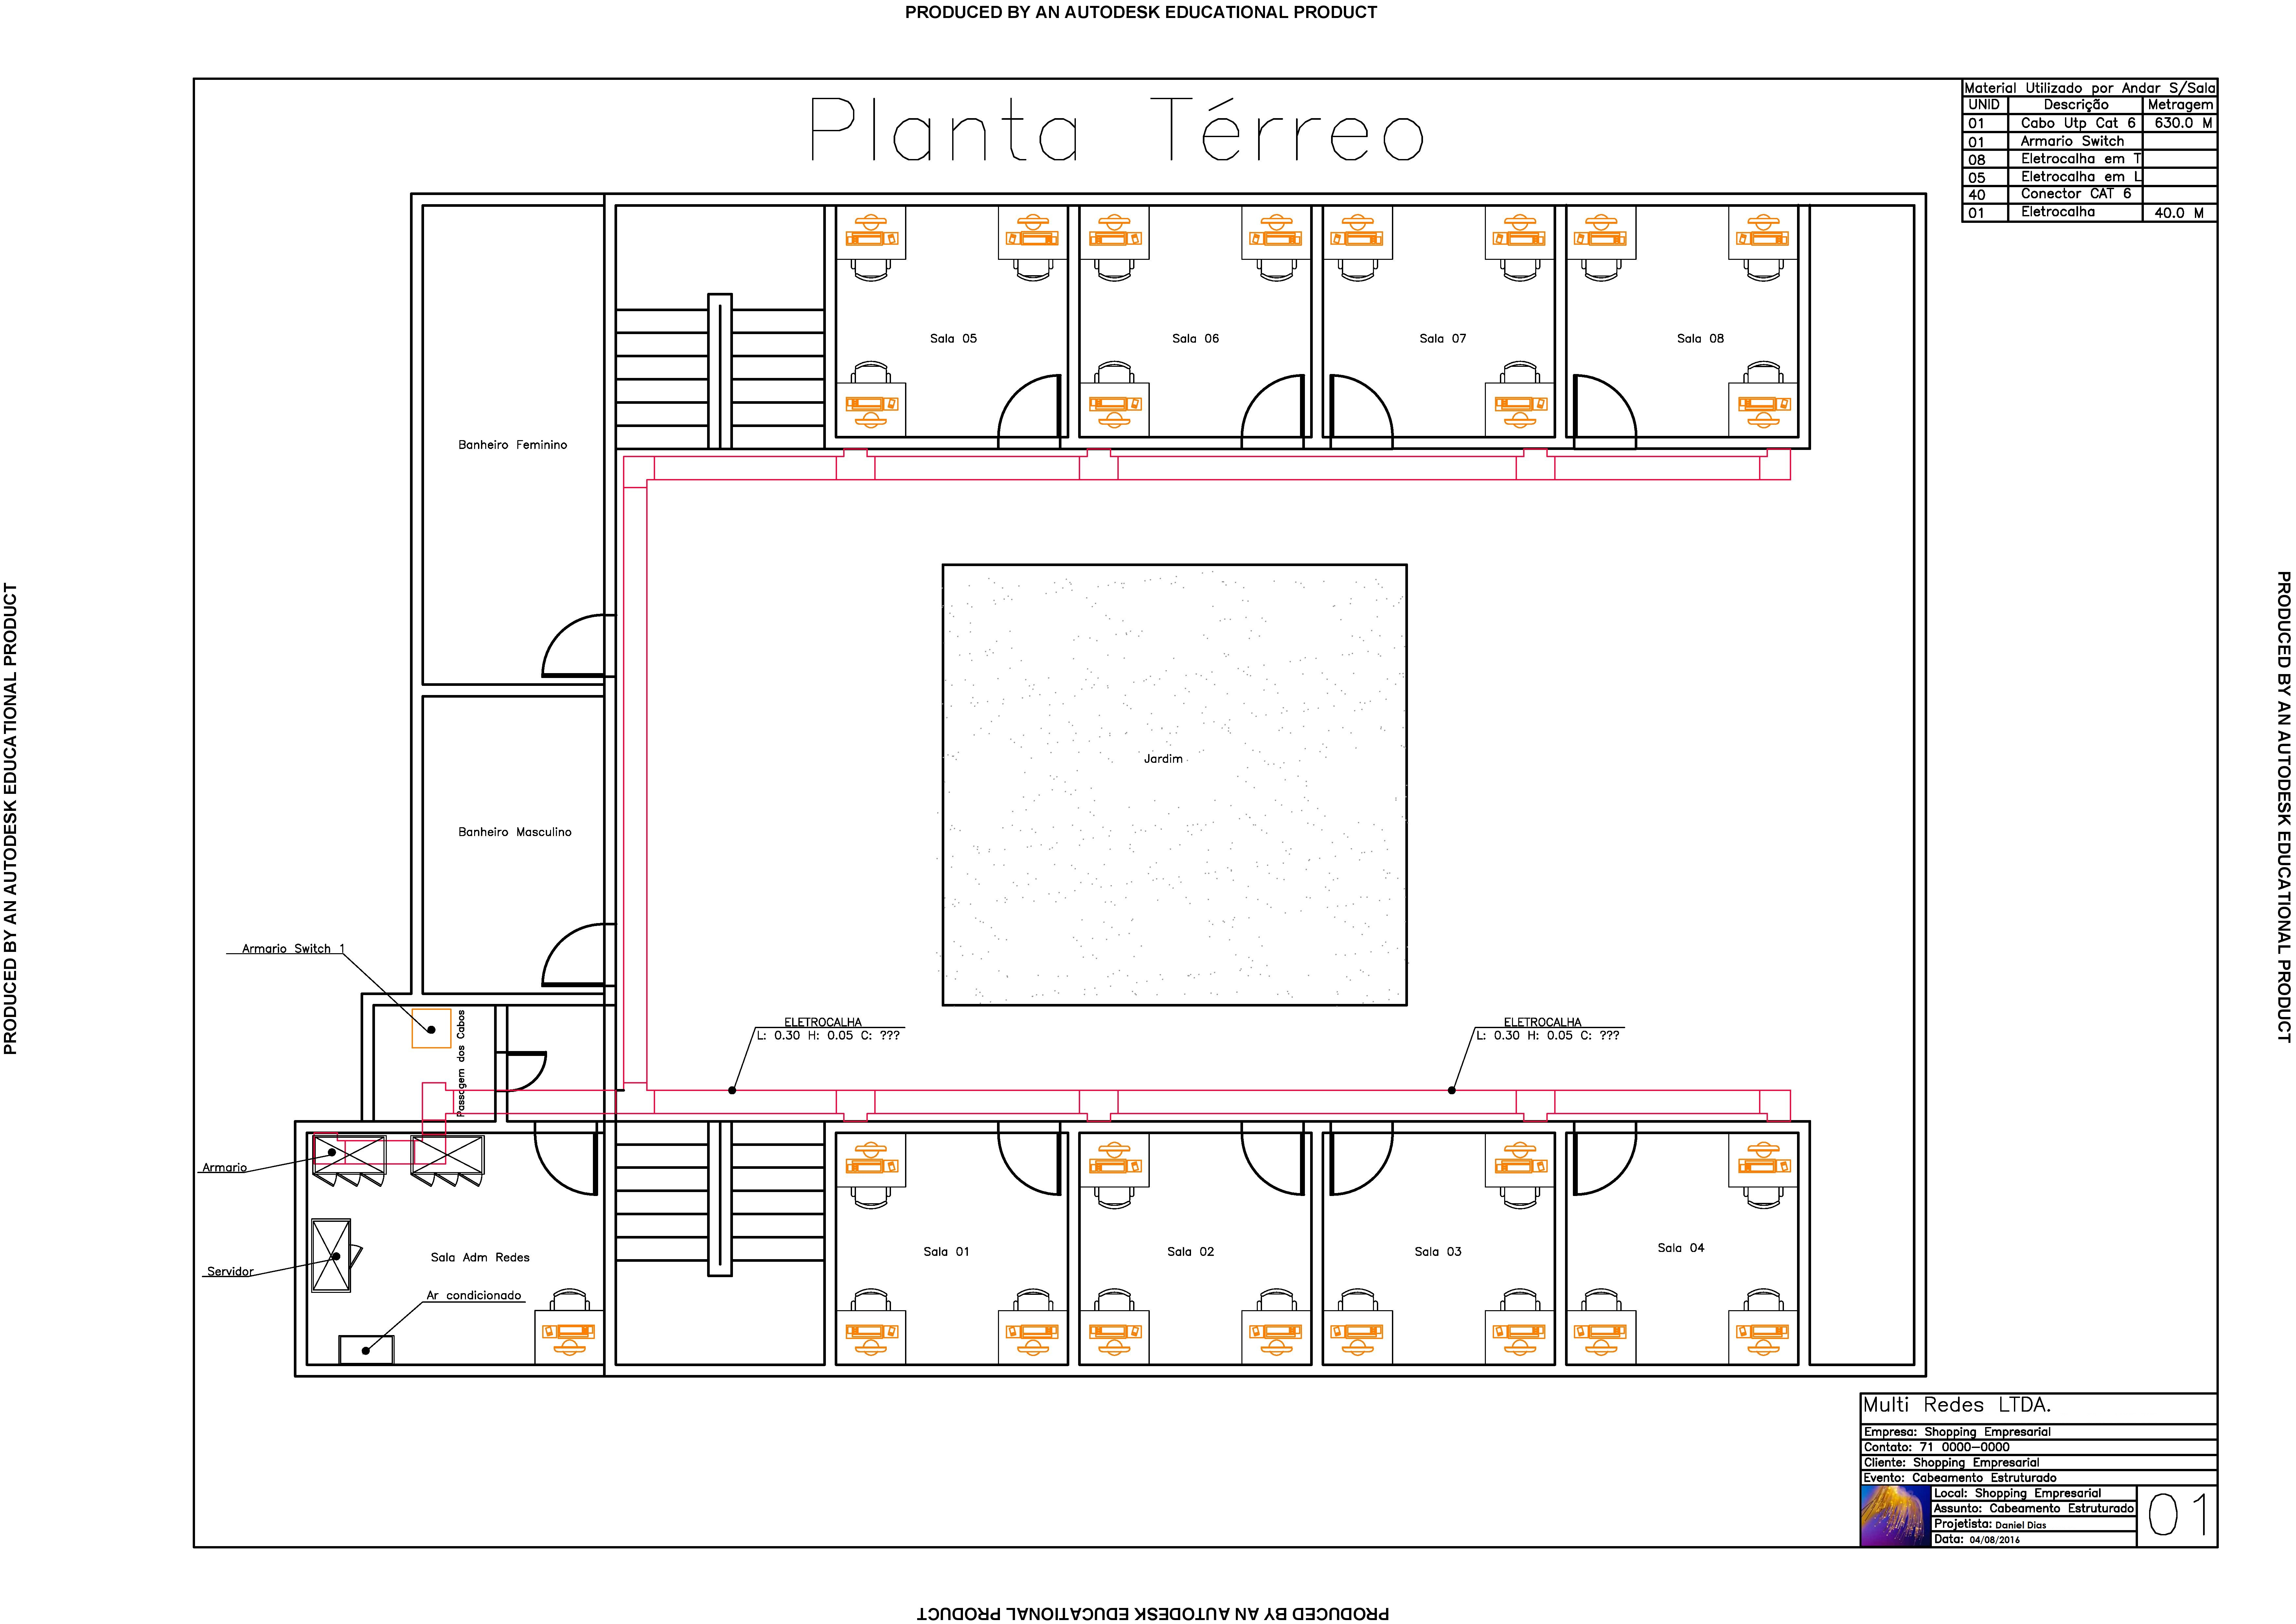
\includegraphics[width=\textwidth]{L1}
\caption{Planta do térreo}
\label{L1}
\end{figure}

\begin{figure}
\centering
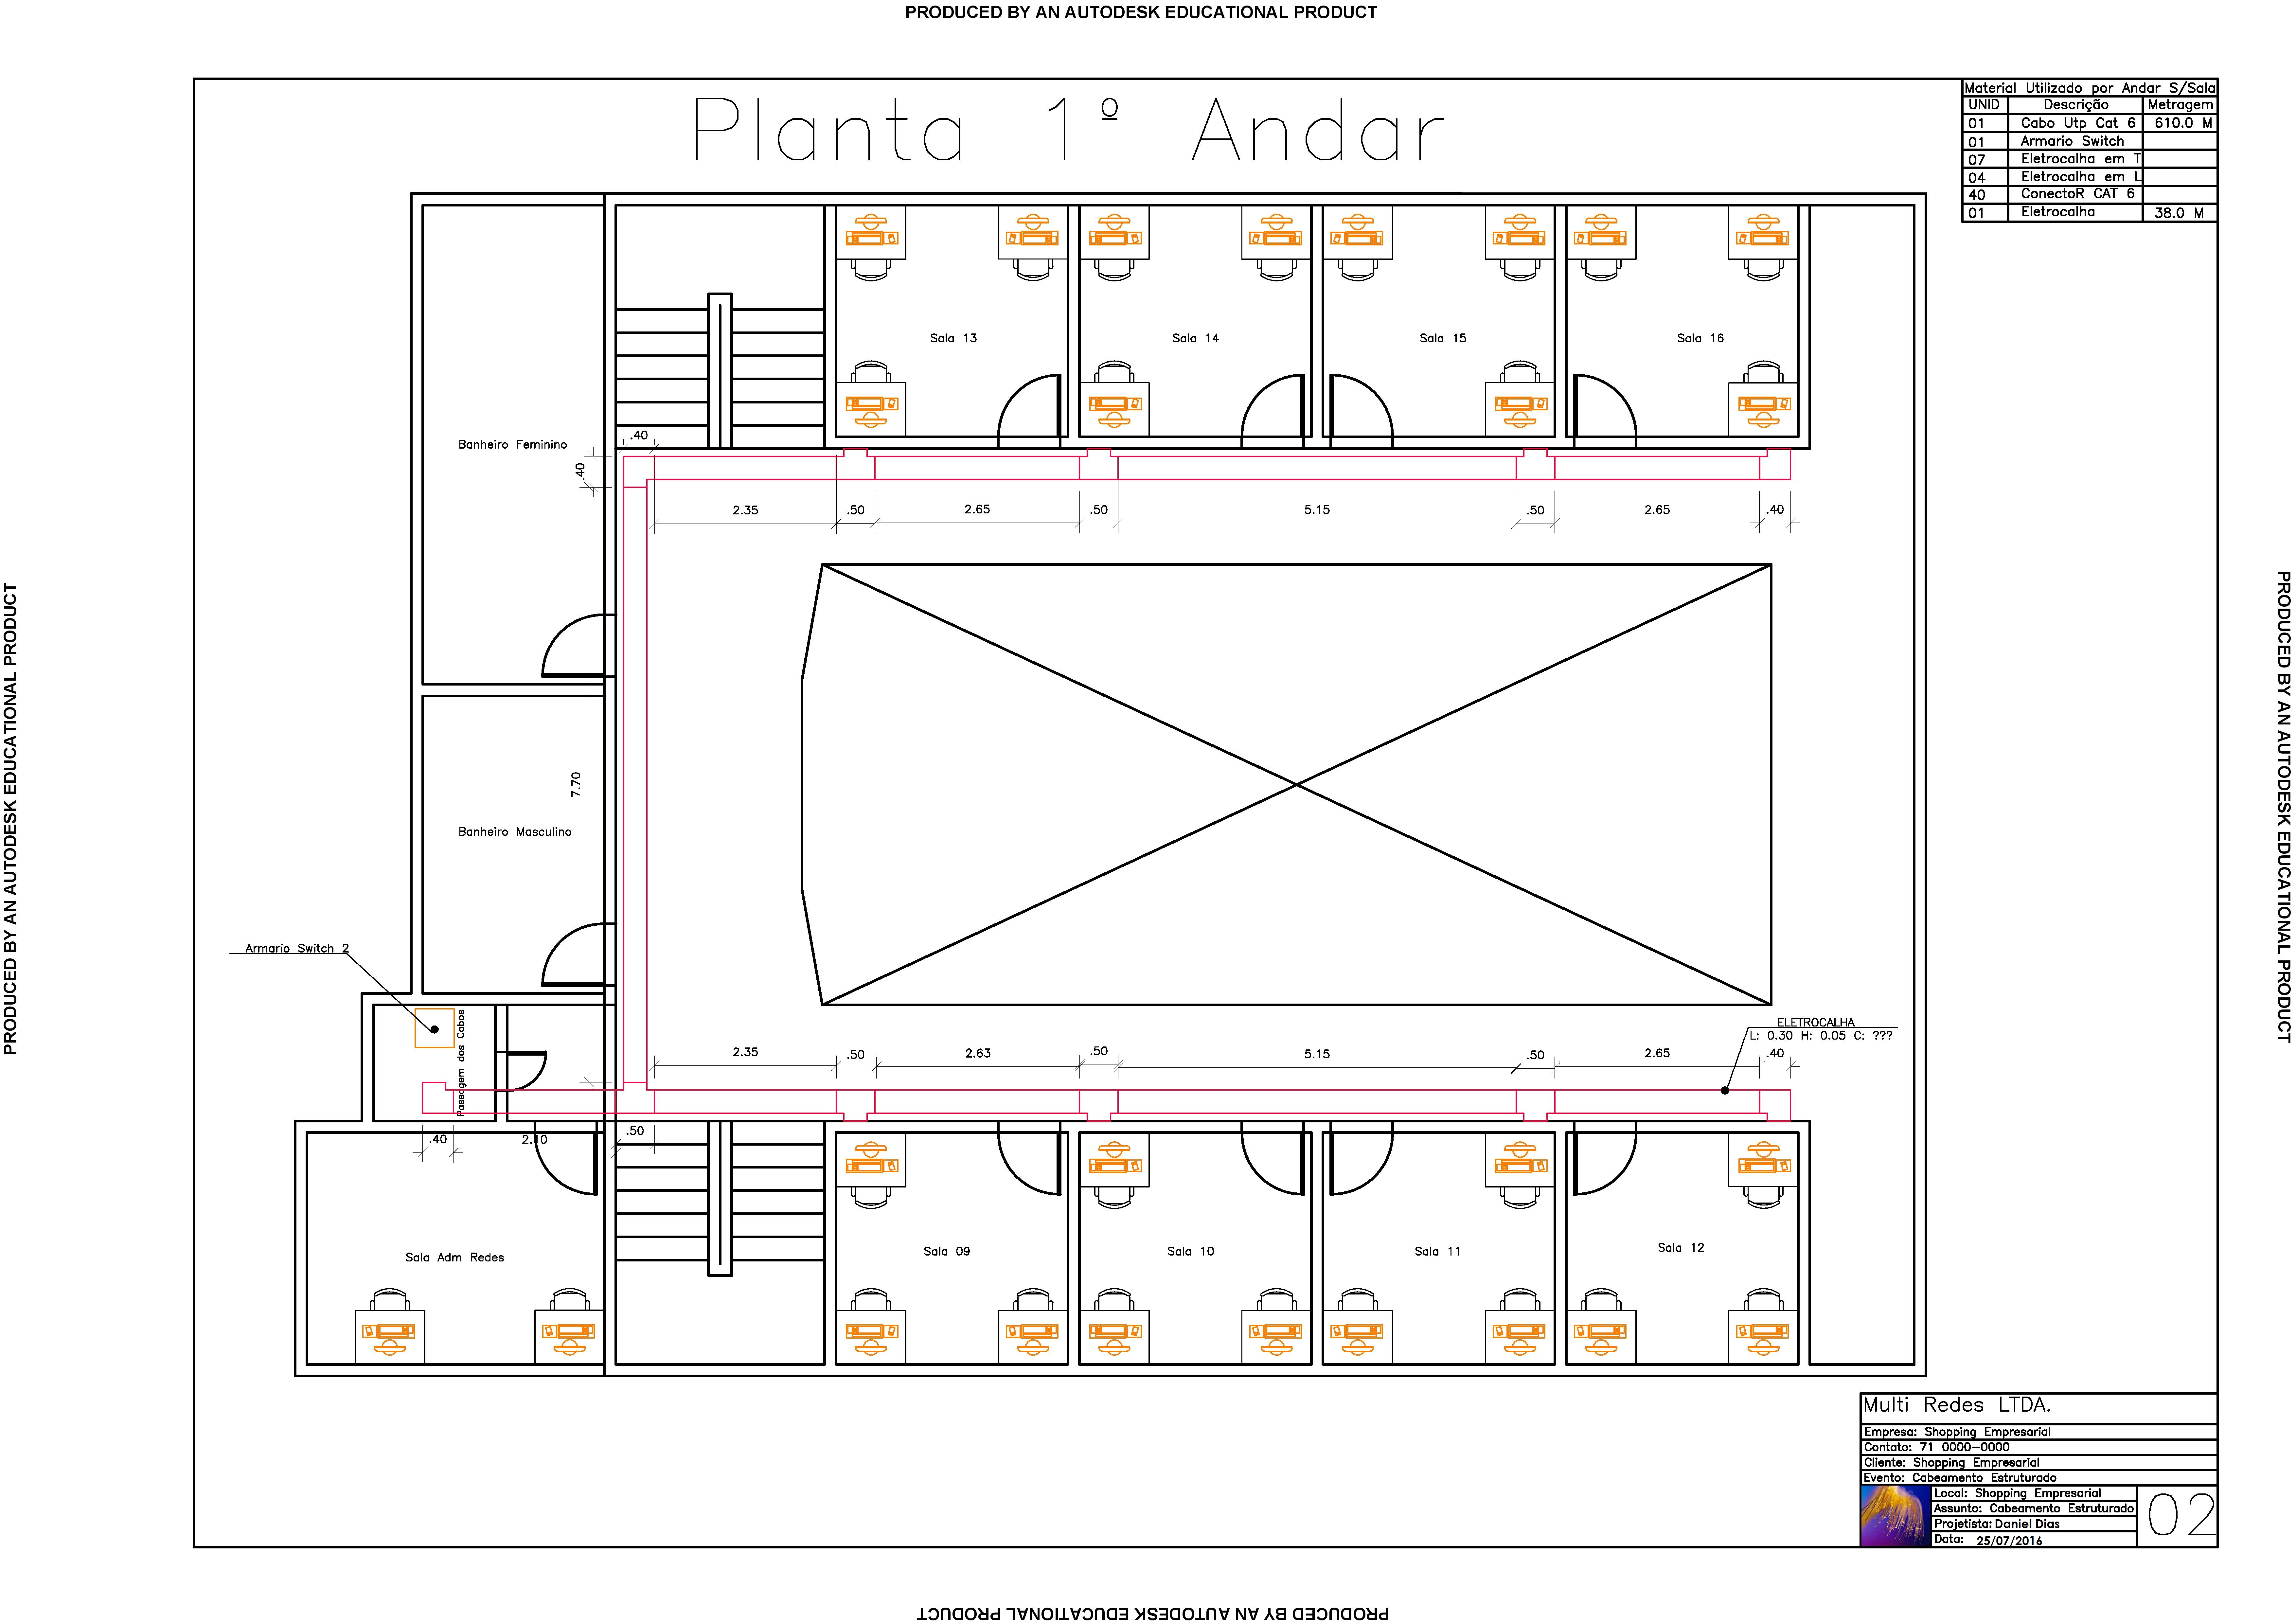
\includegraphics[width=\textwidth]{L3}
\caption{Planta do primeiro andar}
\label{L3}
\end{figure}

O layout das salas para lojistas pode ser verificado na figura \ref{L2}.

\begin{figure}
\centering
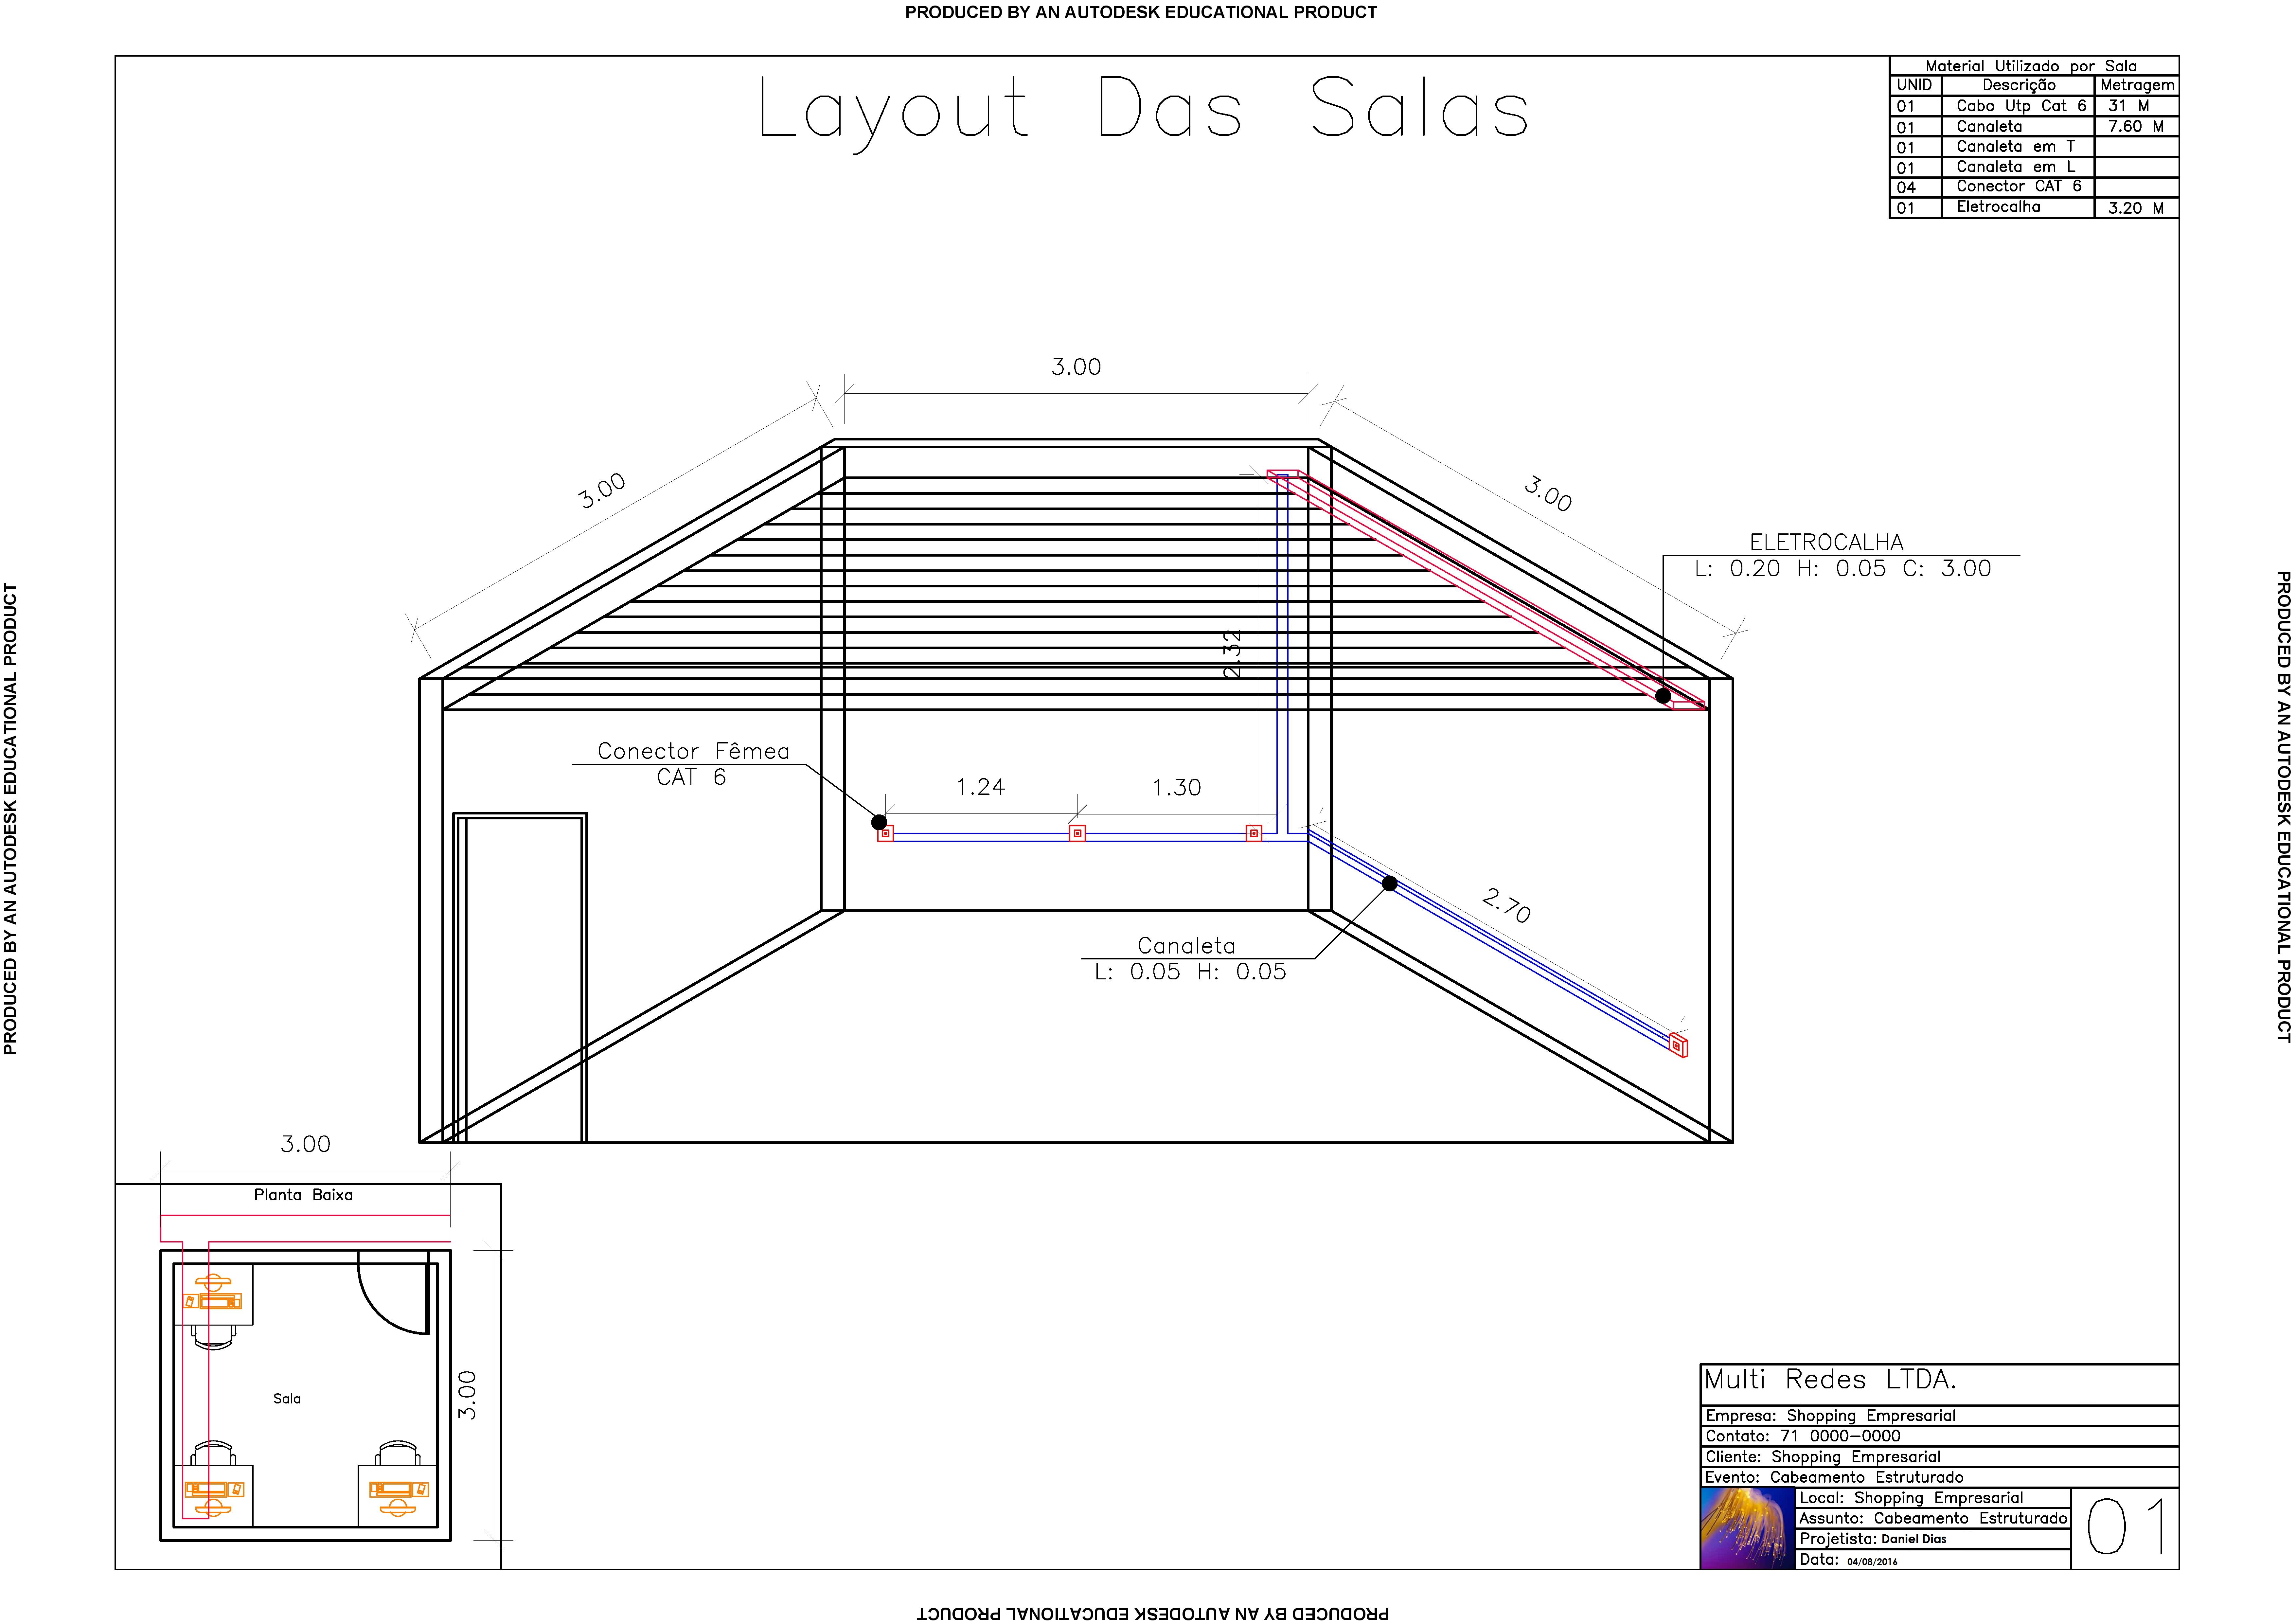
\includegraphics[width=\textwidth]{L2}
\caption{Planta das salas}
\label{L2}
\end{figure}

\section{Planta Lógica - Elementos estruturados}

\subsection{Topologia}
Em sua estrutura a empresa optou por utilizar dois links de internet de igual capacidade para fornecer redundância e segurança aos usuários durante a navegação, L2 em switchs Datacom, com terminações ONU (\textit{Optical Network Unit}) substituindo cabeamento ethernet, L3 com roteador  MX5-Juniper utilizando interfaces de 10Gbps. 
Com a utilização das OLT/ONU, possibilitou uma infraestrutura moderna e extremamente rápida se compararmos aos moldes atuais.
A rede lógica da infraestutura de redes pode ser visualizada na figura \ref{topologia}.
\begin{figure}
\centering
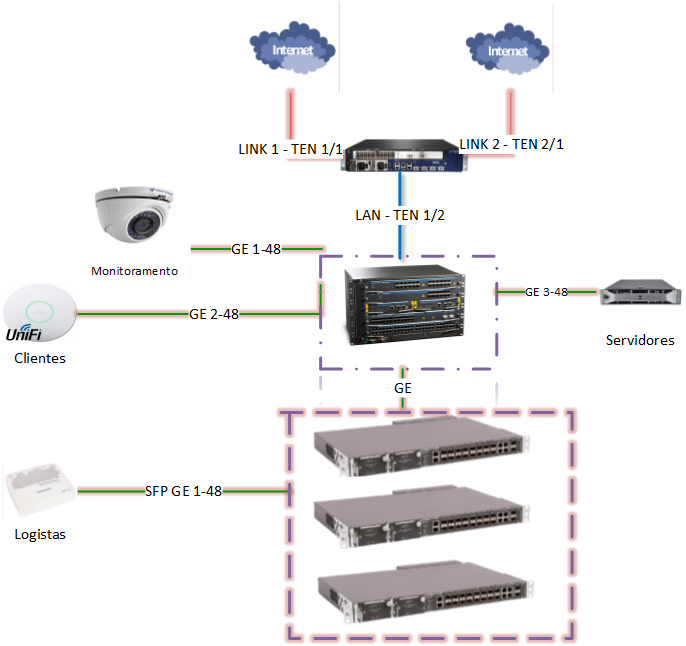
\includegraphics[width=\textwidth]{topologia}
\caption{Topologia de redel}
\label{topologia}
\end{figure}

A visa frontal do rack principal pode ser visualizado na figura \ref{rack}. Nele constam os seguintes equipamentos: Roteadores das operadoras,  router principal, distribuidores opticos, terminadores de linhas opticas, servidor interno, réguas, fonte de alimentação e o inversor para o banco de baterias estacionarias, com as quais garantiremos um fornecimento de energia em caso de interrupções no fornecimento.

\begin{figure}
\centering
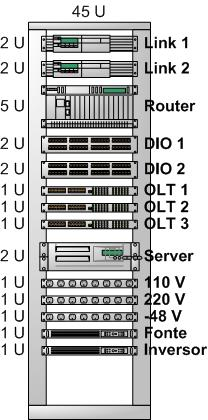
\includegraphics[height=\textwidth]{rack}
\caption{Vista frontal do Rackl}
\label{rack}
\end{figure}


%%Todos os elementos das figuras devem ser explicados. 
%%Crie esboço da configuração dos racks e brackets. Explique cada um dos componentes. Você pode criar uma tabela contendo figuras dentro, ou criar uma tabela e incluí-la como imagem. Por exemplo, verifique a tabela \ref{tab1}.

%%\begin{table}[h!]
\centering
\caption{Exemplo de tabela explicativa}
\label{tab1}
\begin{tabular}{|l|l|l|}
\hline
\multicolumn{3}{|l|}{Figura na Tabela} \\ \hline
1        & Rack          & \includegraphics[scale=0.2]{fig1}        \\ \hline
2        & Rack 2        & \includegraphics[scale=0.2]{fig1}        \\ \hline
\end{tabular}
\end{table}

\subsection{Encaminhamento}
Eletrodutos, calhas, e qualquer material em que os cabos serão alojados/alocados.

\subsection{Memorial descritivo}
%%Relacione todos os equipamentos passivos que serão utilizados, tipo, fabricante, quantidade.

Equipamento passivos utilizados no projeto:
\begin{itemize}
	\item 01 DIO B48  FURUKAWA- Módulo Básico: Responsável por acomodar e proteger a fusão de transição entre o cabo óptico e as extensões ópticas (pigtails) ou para acomodar os cabos pré-conectorizados de fábrica ou conectorizados em campo.  
	\item 04 Patch Panels 24 portas FURUWAKA
	\item 01 Kit Bandeja de Emenda 12F: Responsável por acomodar e proteger as emendas ópticas e o excesso de fibra. Composto por uma bandeja de emenda para até 12/24 fibras fabricada em plástico de alto impacto UL-94 V0.
	\item 01 Kit Placa LGX: Conjunto composto por 3 placas LGX adequadas para instalação em DIOs que suportem a instalação de placa LGX. Disponível em material plástico ou metálico.
	\item 01 Kit Placa LGX - 12 posições SC/APC
	\item 01 Kit de ancoragem e acomodação: Conjunto composto por acessórios de fixação dos cabos ópticos na entrada do DIO. Possibilita mais de duas formas de ancoragem dos cabos.
	\item 01 Extensão Óptica Conectorizada: Cada kit atende 2 ou 6 fibras e é composto por adaptadores ópticos e extensões ópticas. Ideal para aplicações com fusão de fibras no DIO.
	\item 80 Conector Cat6 Fêmea Furukawa
\end{itemize}

\subsection{Identificação dos cabos}

\section{Implantação}

O cronograma de execução das tarefas está de acordo com a figura \ref{tarefas}.

\begin{figure}
\centering
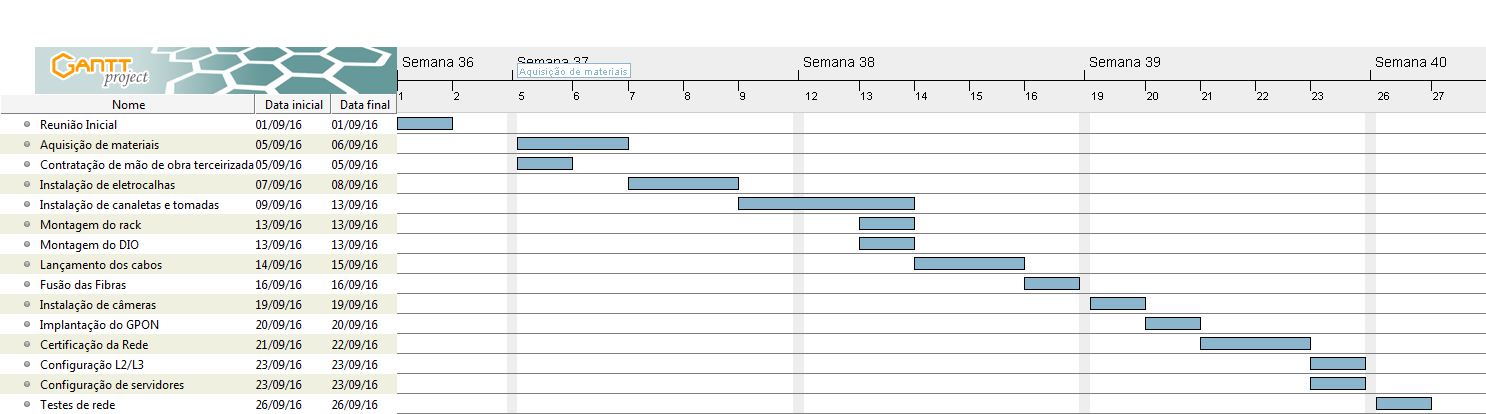
\includegraphics[width=\textwidth]{tarefas}
\caption{Cronograma de execução}
\label{tarefas}
\end{figure}

Na figura \ref{pessoas} estão relacionadas as tarefas e respectivos responsáveis por sua execução.

\begin{figure}
\centering
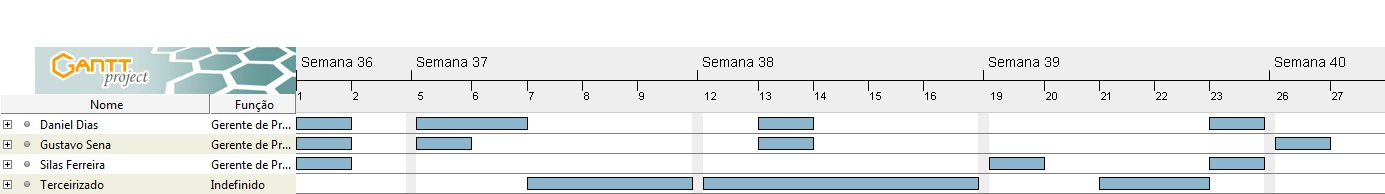
\includegraphics[width=\textwidth]{pessoas}
\caption{Pessoas e atividades}
\label{pessoas}
\end{figure}
%%Estabeleça um cronograma de implantação:
%%Remoção de equipamentos existentes (destino para descarte), instalação dos condutores, instalação dos cabos, 
%%identificação dos cabos, montagem dos racks, certificação, etc... Crie atividades e estabeleça o tempo de execução. Se for um projeto real, indique também quais os responsáveis pela execução do projeto e de cada uma das etapas.

%%Defina marcas (e padrões) e fornecedores se for o caso. Atenção a contratados e subcontratados para a realização das atividades. Estabeleça a responsabilidade de execução da atividade e também da validação dela.
%%
%%Utilize algum software para gerear o cronograma. Excel,etc. O fundamental é dividir em etapas, descrever e estimar o tempo de cada uma delas.

%%Segue uma relação de ferramentas:
%%http://asana.com/, 
%%https://trello.com/, 
%%http://www.ganttproject.biz/, 
%%http://www.orangescrum.org/. 

\section{Plano de certificação}
De modo a assegurar a qualidade do projeto, será realizada a certificação tanto do cabeamento óptico quanto do elétrico de toda a infraestrutura.
A certificação irá ocorrer após a realização das atividades relacionadas ao cabeamento e antes da configuração e testes de rede.
Antes de realizar a certificação é necessário a identificação precisa do tipo de fibra e da aplicação projetada, pois só assim será possível validar ou não a qualidade do cabeamento
de acordo com os valores de referência para distância máxima e atenuação das normas TIA 568C e IEC 11801. 

\subsection{Cabeamento Óptico}
Para a certificação óptica será executados testes de Nível 1 e 2 de acordo com as boas práticas especificadas em \cite{ref6}.
\subsubsection{Nível 1: OLTS (\textit{Optical Loss Test Set})}
\begin{itemize}
	\item Teste realizado utilizando-se um \textit{Power Meter}
	\item Verifica a perda óptica do cabeamento, seu comprimento e polarização
\end{itemize}

\subsubsection{Nível 2: \textit{Tier}1 mais um traço de OTDR (\textit{Optical Time-domain Reflectometer})}
\begin{itemize}
	\item Teste realizado utilizando-se um OTRD
	\item Verificação atenuação uniforme do cabo e perda da inserção de conectores
	\item Teste mais detalhado, provendo informações quantitativas quanto ao desempenho do sistema de cabeamento e seus componentes
\end{itemize}

\subsection{Cabeamento Elétrico}
Para o cabeamento elétrico, seguindo as boas práticas em \cite{ref6}, será realizado testes de canal (enlace) utilizando um scanner.
Os testes de enlace foram escolhidos por serem mais completos, pois compreendem todos os componentes do cabeamento (parte fixa e patch chords).
As seguintes caractéristicas serão testadas:
\begin{itemize}
	\item Impedância
	\item Atenuação
	\item Paradiafonia (interferência entre pares de fios)
	\item Perda de retorno
	\item Tempo de propagação
	\item ACR (\textit{Atenuation to Crosstalk Ratio})
\end{itemize}

Quais seriam as etapas para a certificação? 
Quais os locais e horários para execução da certificação na rede? Toda rede será certificada?
Como os testes seriam executados?
Quais relatórios de certificação serão (ou deveriam ser) entregues? 

\section{Plano de manutenção}

Considerando-se que o projeto só será entregue após obter resultados positivos da certificação da rede, a manutenção da rede seguirá uma abordagem corretiva.
A partir do momento que a rede estiver em operação, esta será monitorada continuamente pela equipe de TI através da utilização de ferramentas específicas que suportem o protocolo SNMP (\textit{Simple Network Management Protocol}).
Assim será possível identificar possíveis problemas, os quais podem requerer uma análise mais minuciosa, podendo ou não levar à substituição de algum componente do cabeamento.


\subsection{Plano de expansão}
Existe um plano de expansão? Quantos novos pontos poderão ser acrecidos na rede, antes de migração de equipamentos na camada 2? Se houver expansão, quais equipamentos deverão ser direcionados para as estremidades da rede? 


\section{Orçamento}
Crie uma relação de orçamentos baseado na seções anteriores.





\section{Referências bibliográficas}
%%Utilize o mendley, o jabref ou diretamente o bibtex para gerenciar suas referências biliográficas. As referências são criadas automaticamente de acordo com o uso no texto.

%%Exemplo: Redes de computadores, segundo \cite{t2013} é considerada..... Já \cite{kurose2010} apresenta uma versão...

%%Analisando os pressupostos de \cite{ref3} e \cite{ref4} concluimos que....


\renewcommand\refname{} %%Referências bibliográficas}  
\bibliographystyle{ieeetr}
\bibliography{referencias}  

%% ***********************************************************************
%% === remover daqui =====================================================
%% ***********************************************************************

%%\section{Elementos textuais - Alguns exemplos}

%%Esta seção apresenta exemplos de elementos textuais. \textbf{Remova-a da versão final do texto}.


%%\subsection{Colocar elementos em itens}
%%Texto antes da lista
%%
%%\begin{itemize}
%%	\item First item in a list 
%%	\item Second item in a list 
%%	\item Third item in a list
%%\end{itemize}

%%\subsubsection{Uma sub seçao de terceiro nivel}

%%Exemplo de uma subseção

%%\subsection{Tabelas}

%%Utilize o site http://www.tablesgenerator.com/ para elaborar as tabelas de seu trabalho.
%%Para adicionar uma tabela utilize: a tag input, passando o arquivo da tabela como parametro

%%\begin{table}[h!] % coloque h! para forcar a posicao
\centering
\caption{Modifique a legenda e crie um label}
\label{tab2} %com este label vc faz referencia no texto
\begin{tabular}{|l|l|l|l|l|}
\hline
\multicolumn{1}{|c|}{\textbf{Este é um exemplo de tabela}} & \multicolumn{2}{c|}{\textbf{C1}} & \multicolumn{2}{c|}{\textbf{C2}} \\ \hline
Você pode criar a tabela no excel                          & 1              & 2               & 3               & 4              \\ \hline
Exportar para CSV                                          & 5              & 6               & 7               & 8              \\ \hline
E importar no Table Generator                              & 9              & 10              &                 &                \\ \hline
\multicolumn{5}{|c|}{\textit{Gere o tex, e adicione em seu arquivo}}                                                             \\ \hline
\end{tabular}
\end{table}

%%Dentro do arquivo você deve definir o label e pode utilizá-lo para referenciar. Exemplo:
%%Na tab \ref{tab2} temos a relação de ....


%%Você também pode modificar a tabela manualmente, incluindo, por exemplo h! dentro de sua definição. Veja no exemplo tab2.tex

%%\subsection{Figuras}

%%As figuras podem ser no formato PDF, JPG, PNG. Você pode referenciá-las da mesma maneira que tabelas. Exemplo: A figura \ref{fig1} apresenta.....
%
%%Não se preocupe o local em que a figura será renderizada em seu texto. Preocupe-se em criar referência para ela, ou seja, toda figura e tabela deve conter pelo menos uma referência no texto.

%%\begin{figure}
%%\centering
%%\includegraphics[width=\textwidth]{fig1}
%%\caption{Exemplo de figura com escala horizontal}
%%\label{fig1}
%%\end{figure}


%%\begin{figure}
%%	\centering%%
%%	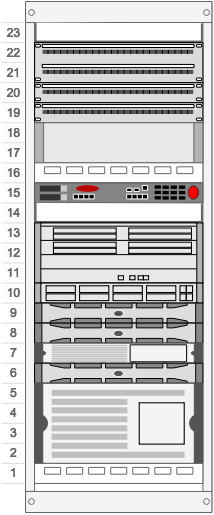
\includegraphics[]{fig2}
%%	\caption{Exemplo de figura sem escala}
%%	\label{fig2}
%%\end{figure}

%%Você pode rotacionar figuras também. Para isso utilize o parâmetro angle=-90. Repare que a escala da figura foi modificada pelo parametro height. Você também pode utilizar scale
%%
%%\begin{figure}
%%	\centering
%%	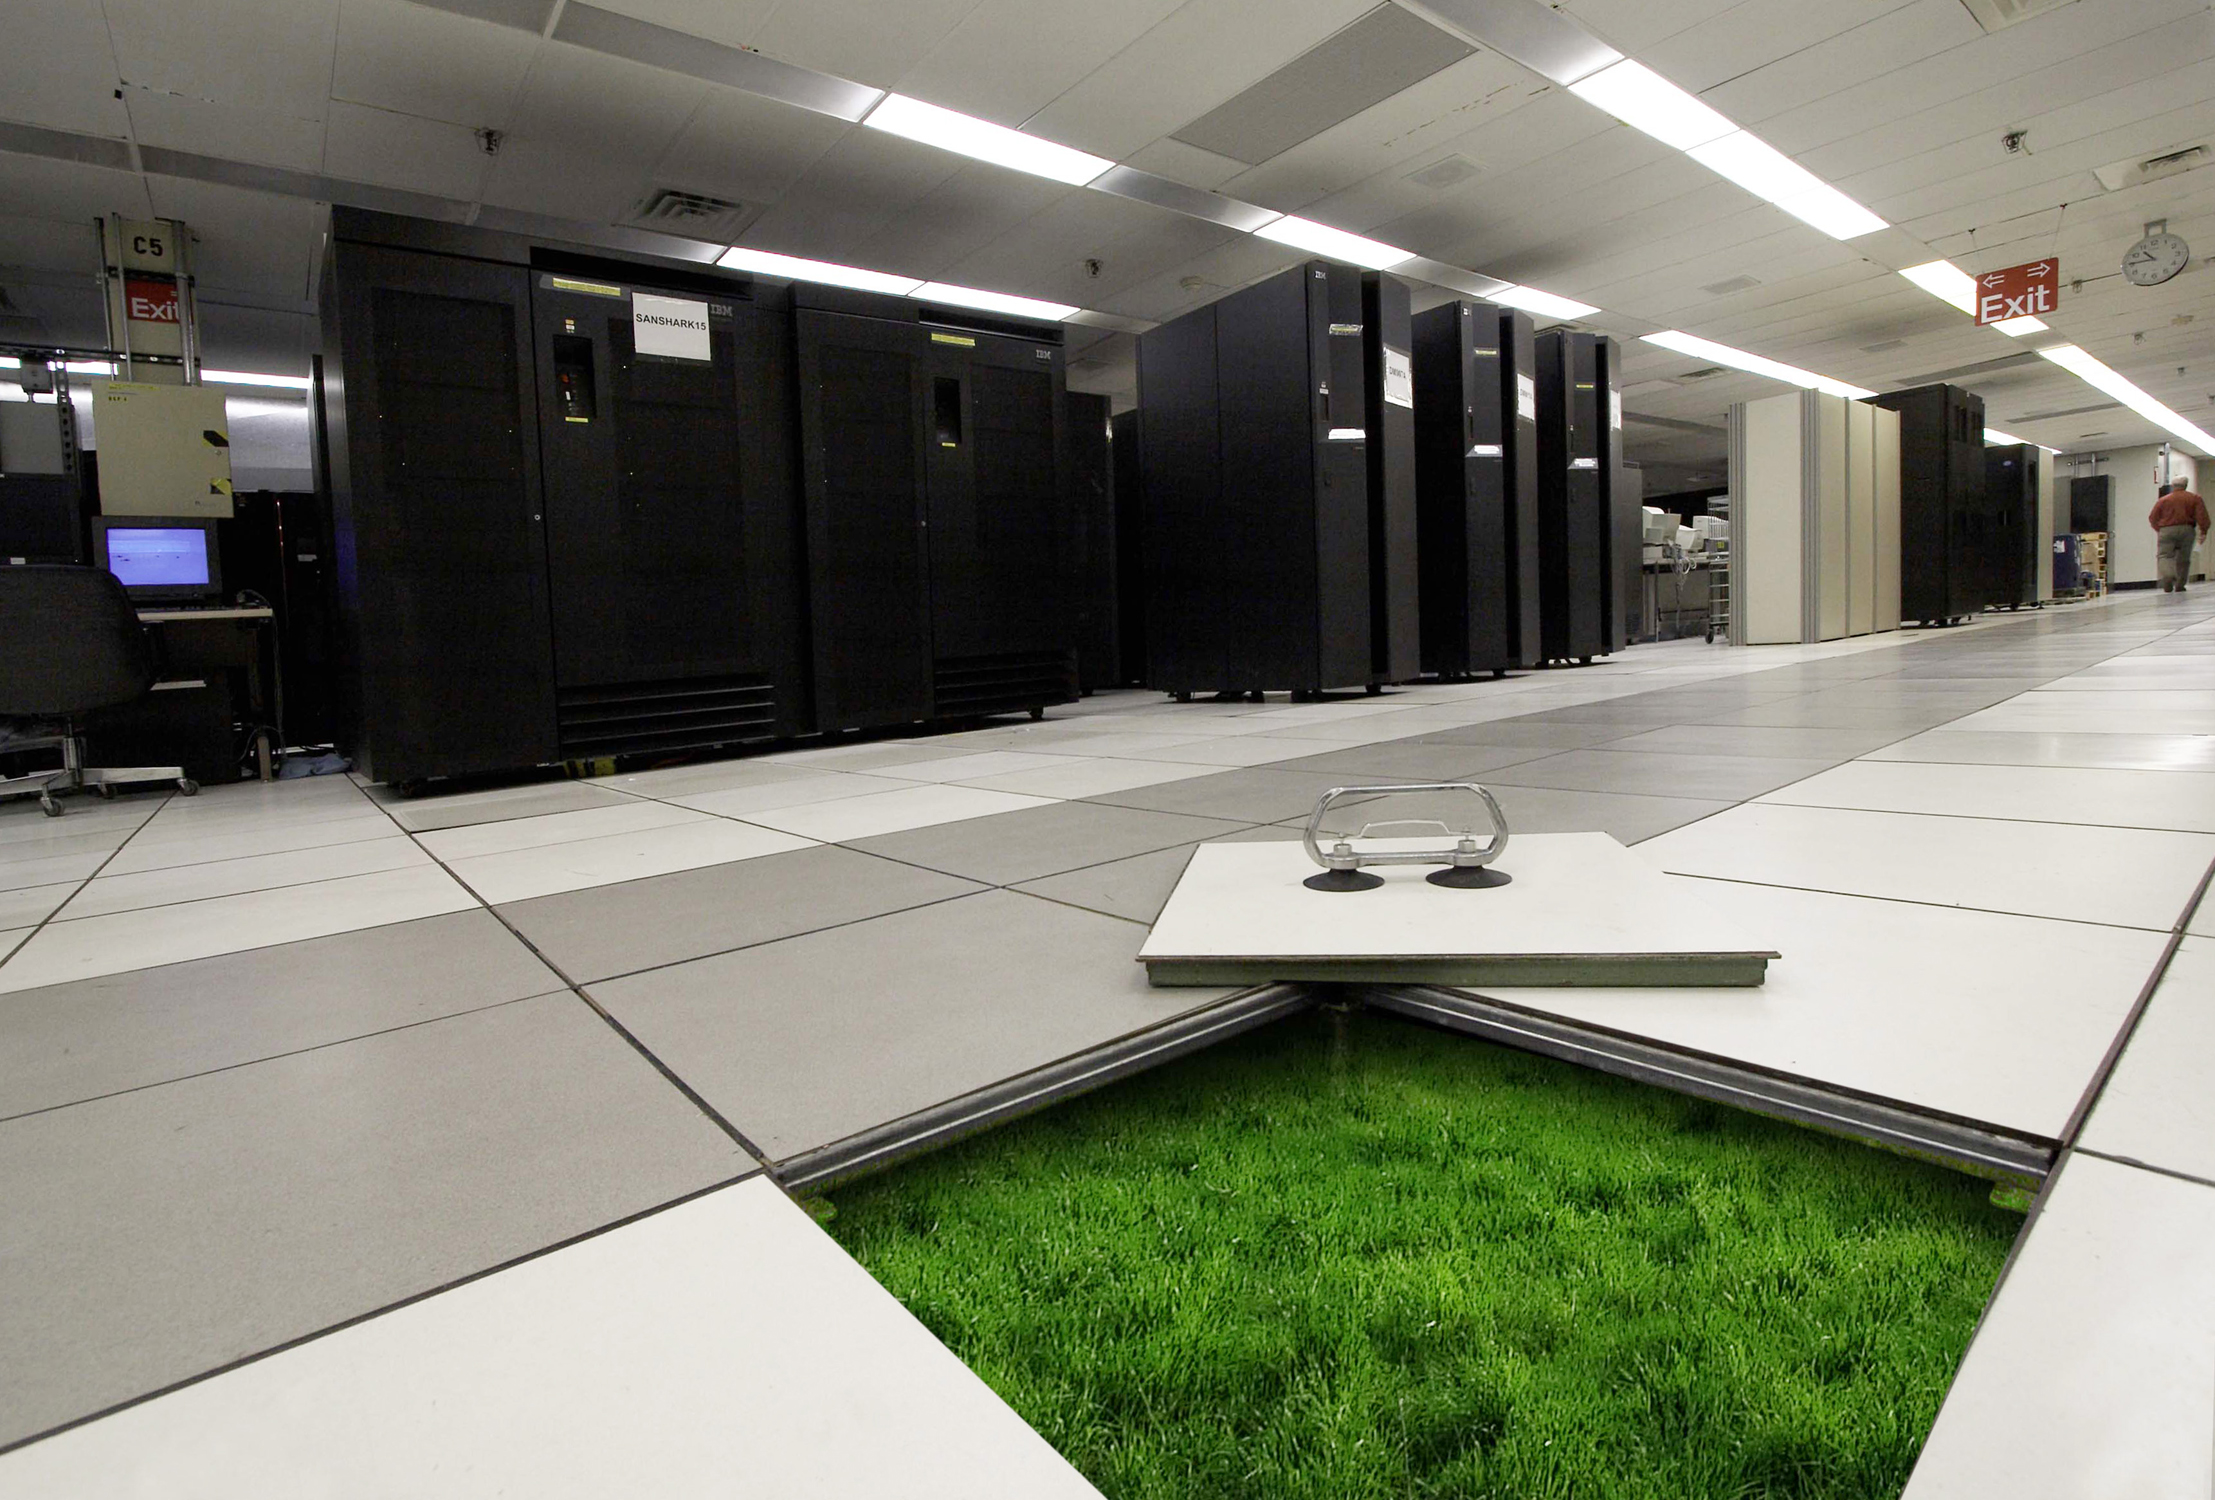
\includegraphics[height=\textwidth,angle=-90]{fig3}
%%	\caption{Exemplo de figura rotacionada}
%%	\label{fig3}
%%\end{figure}


%% ***********************************************************************
%% === ate aqui    =====  ================================================
%% ***********************************************************************
\end{document}